\documentclass{article}
\usepackage[utf8]{inputenc}
\usepackage[legalpaper, portrait, margin=1in]{geometry}
\usepackage{enumitem}
\usepackage{graphicx}


\title{CS 156a Set 4}
\author{Cason Shepard}
\date\today

\begin{document}

\maketitle

\section*{problem 1}
By plugging in $\epsilon = 0.05$ and $\delta = 0.05$, we get the expression:
\begin{center}
    $\epsilon = \sqrt{\frac{8}{N} * ln\frac{4m_H(2N)}{\delta}}$\\
    $0.05 = \sqrt{\frac{8}{N} * ln\frac{4m_H(2N)}{0.05}}$\\
\end{center}
Solving for N, gives us $N = 453000$, which is closest to 460000.\\\\
\textbf{The answer is [d]}

\section*{problem 2}
Devrone's bound does not appear in Desmos, but it is .215 upon calculation as depicted on the graph below:
\begin{center}
    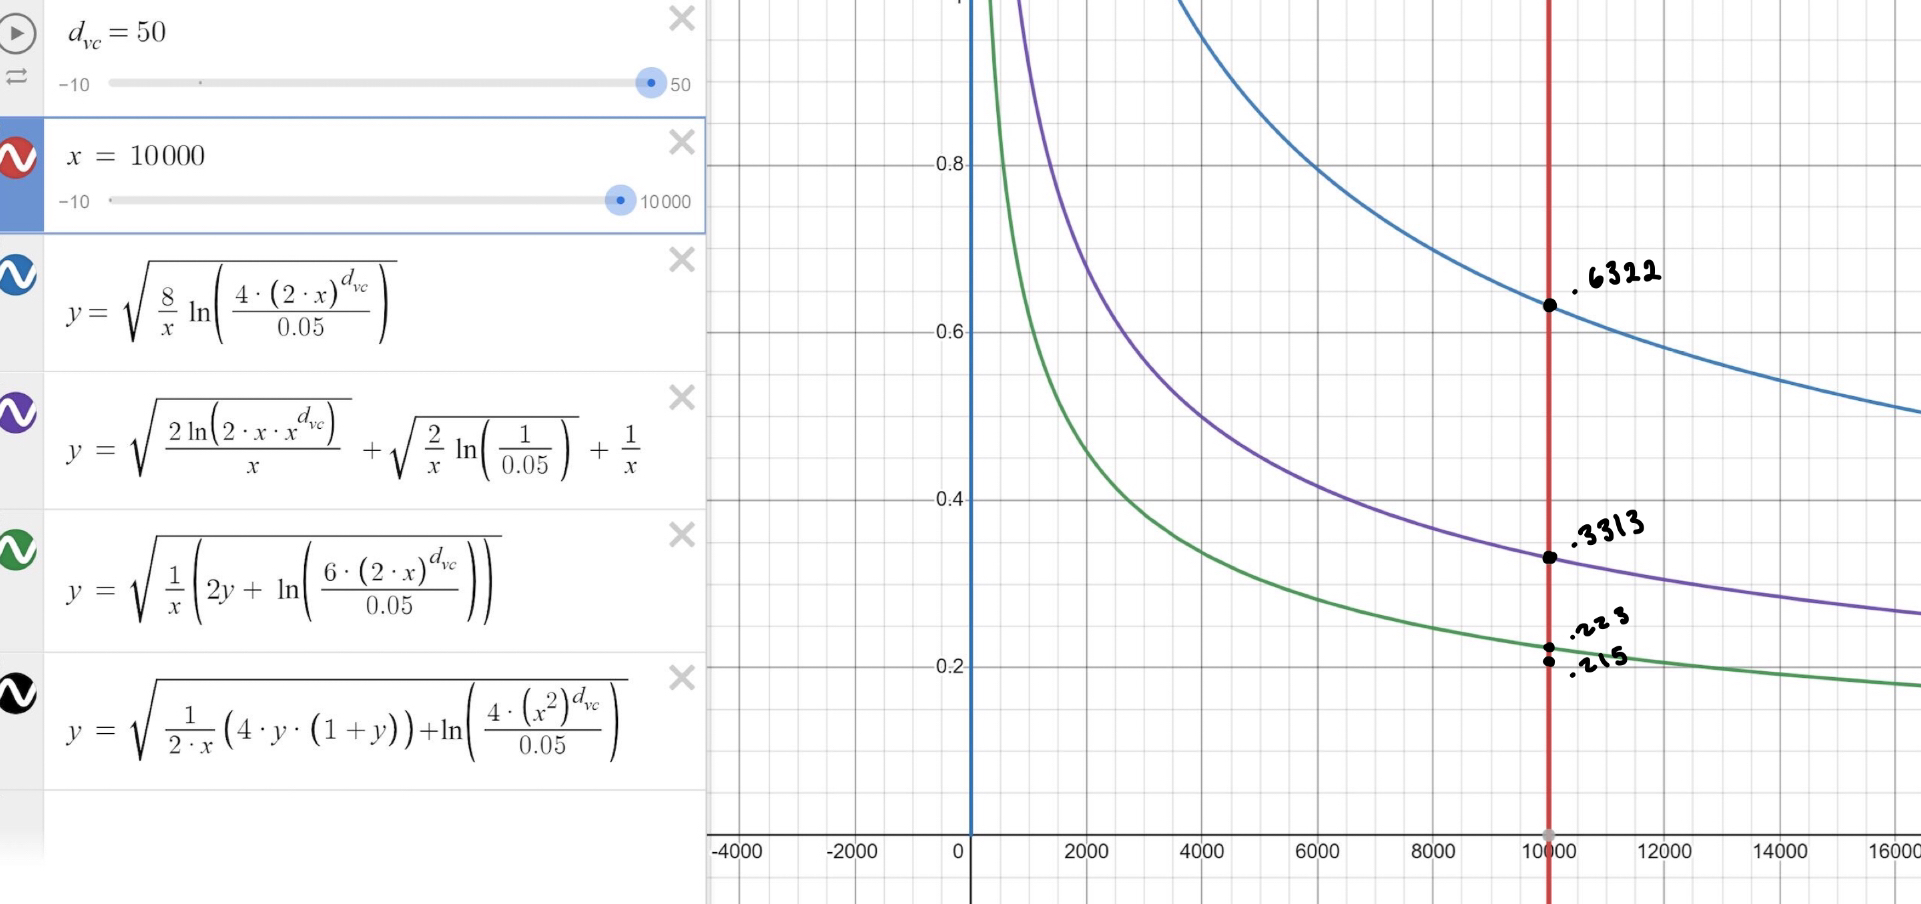
\includegraphics[width=400]{desmoscs156prob2.jpg}
\end{center}
\textbf{The answer is [d]}

\section*{problem 3}
Parrondo and Van den Broek's bound is the smallest at $N=5$ with a value of 5.101.
\begin{center}
    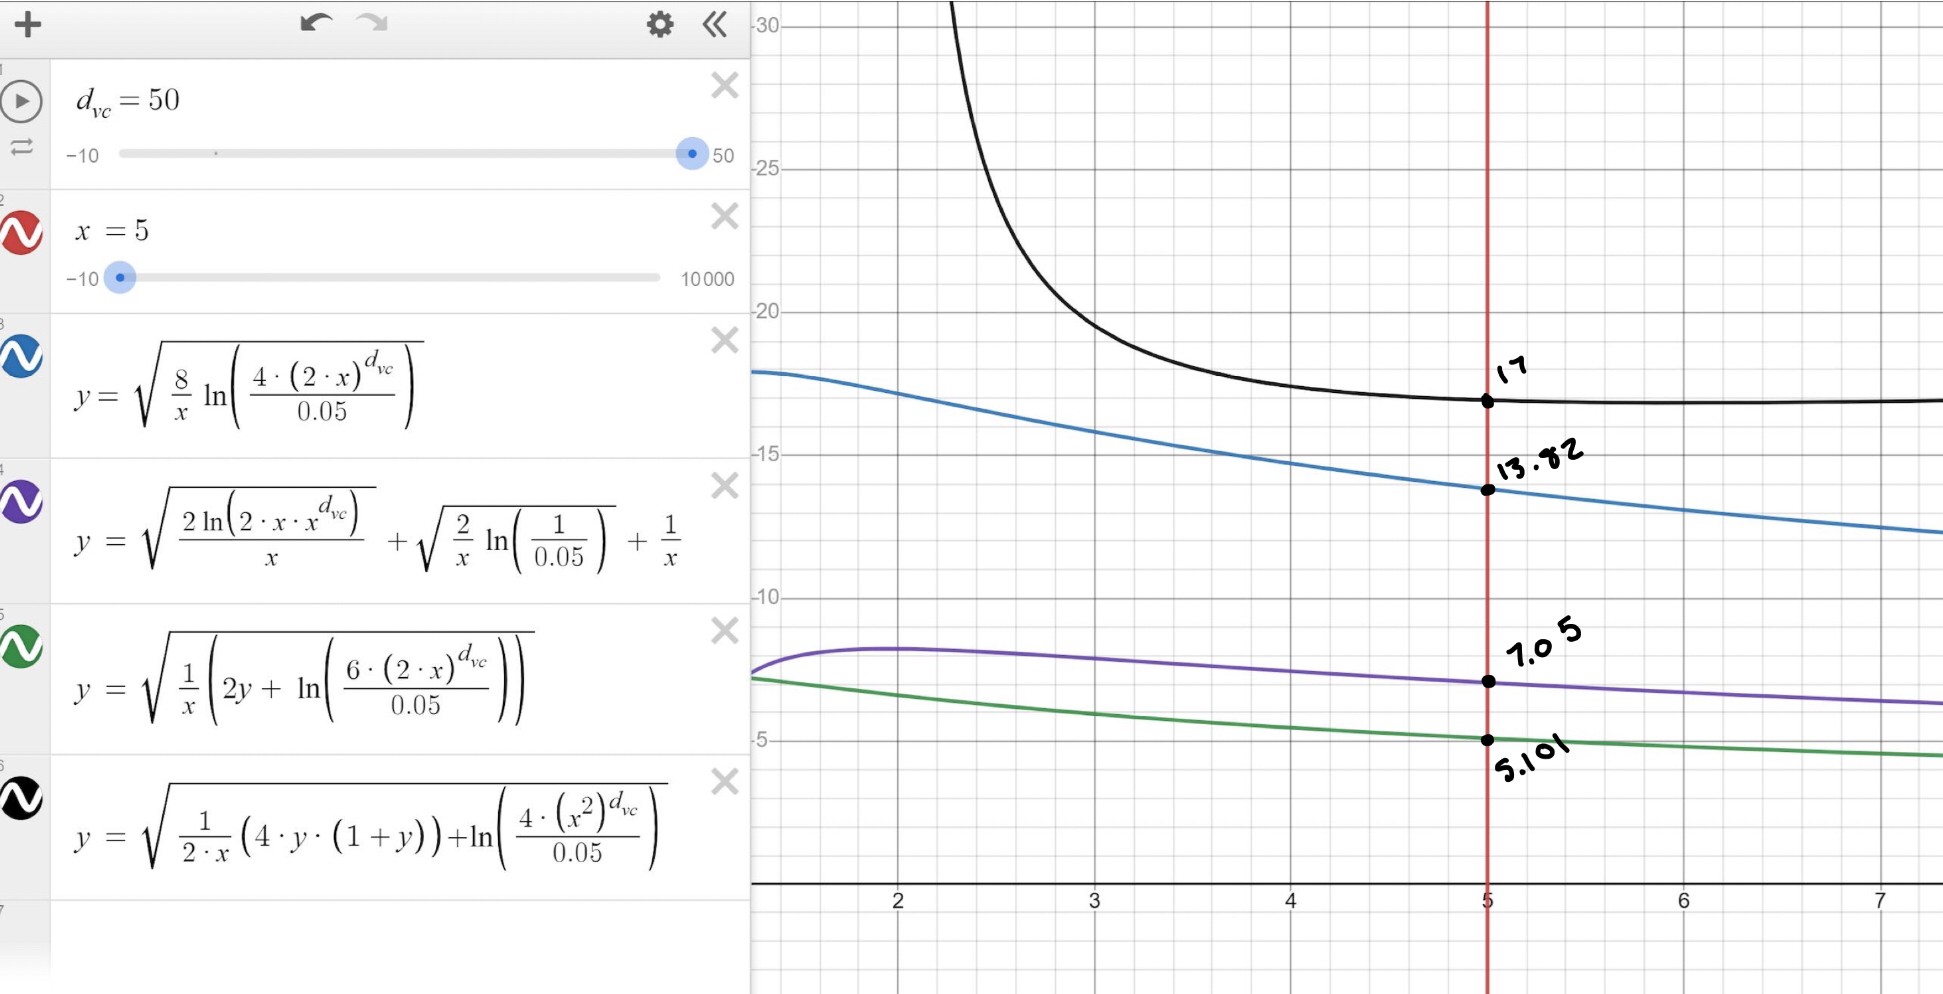
\includegraphics[width=400]{cs156prob3set4.jpg}
\end{center}
\textbf{The answer is [c]}
\newpage
{\huge The following algorithm was used for problems 4-6:}
\begin{verbatim}
import random
import math
from random import uniform
import random

def f(x):
    return math.sin(math.pi*x)

def rand_slope():
    x_1 = uniform(-1, 1)
    x_2 = uniform(-1, 1)
    y_1 = f(x_1)
    y_2 = f(x_2)
    a = ((x_1 * y_1) + (x_2 * y_2)) / (x_1**2 + x_2**2)
    return a   

N = 100000
a_avg = 0

for x in range(N):
    a = rand_slope()
    a_avg += a

a_avg /= N

N_points = 100000
deviation_sum = 0
for x in range(N_points):
    p = uniform(-1, 1)
    deviation_sum += (a_avg*p - f(p))**2

N_slopes = 100000
slope_var = 0
for x in range(N_slopes):
    slope = rand_slope()
    q = uniform(-1, 1)
    slope_var += (a_avg*q - slope*q)**2

print(f"Bias: {deviation_sum/N_points}, Variance: {slope_var/N_slopes}.")
\end{verbatim}
\section*{problem 4}
In order to find the least squares regression of the form $g(x) = ax$, we needed to use the Ordinary Least Squares formula:
\begin{center}
    $a = \frac{\sum^N_{i=1}x_iy_i}{\sum_{i=1}^Nx_i^2}$
\end{center}
After 100000 iterations, the average value for a was 1.42, which is not an option.\\\\
\textbf{The answer is [e]}

\section*{problem 5}
After calculating the bias on 100000 points, the average bias was .27, which is closest to .3.\\\\
\textbf{The answer is [b]}

\section*{problem 6}
After calculating the variance on 100000 points, the average variance was .23, which is closest to .2.\\\\
\textbf{The answer is [a]}

\section*{problem 7}
For each option below, my algorithm was run with the hypothesis function given and averaged over 100000 iterations. 
\begin{enumerate}[label=(\alph*)]
    \item $h(x) = b$, $E_{out} = .5 + .25 = .75$
    \item $h(x) = ax$, $E_{out} = .27 + .23 = .5$
    \item $h(x) = ax + b$, $E_{out} = .21 + 1.68 = 1.89$
\end{enumerate}
For options d and e, we know that the $E_{out}$ will not be lower than those hypothesis functions that have already been tested, thus, we do not need to test them.\\\\
\textbf{The answer is [b]}

\section*{problem 8}
To find the VC dimension for this hypothesis set, we must find when the growth function diverges from the binary classification growth function where $m_H(N) = 2^N$.
\begin{center}
    $m_H(N+1) = 2m_H(N) - {N\choose q}$\\
    $2^{N+1} = 2 * 2^N - {N \choose q}$\\
    $2^{N+1} = 2^{N+1} - {N\choose q}$
\end{center}
We now see that the divergence depends on when ${N\choose q}\neq 0$. However, if we first set ${N\choose q} = 0$, we find that $N \leq q-1$. We then get:
\begin{center}
    $2^{N+1} = 2^{N+1} - {q-1\choose q}$\\
    $2^{N+1} = 2^{N+1} - 0$
\end{center}
However, we can increment $q-1 \rightarrow q$ to get:
\begin{center}
    $2^{N+1} = 2^{N+1} - {q\choose q}$\\
    $2^{N+1} = 2^{N+1} - 1$
\end{center}
At $N=q$, the growth function for this hypothesis set begins to diverge, and thus the VC dimension is q.\\\\
\textbf{The answer is [c]}

\section*{problem 9}
We know that since the $d_{VC}$ of an empty hypothesis set is 0, our lower bound for this intersection of hypothesis sets (disjoint sets) must be 0, which rules out d and e as possible solutions. This leaves a, b, and c as possible solutions. Since we are looking for the tightest bound, b is the correct solution. We can rule out c as this bounds $d_{VC}$ under the maximum VC dimension able to be shattered by any hypothesis set $H_k$. This is incorrect as the hypothesis sets may not be identical, causing this bound to be too loose. We can also rule out a, as the upper bound of this option is not tight enough.\\\\
\textbf{The answer is [b]}

\section*{problem 10}
\textbf{The answer is []}

\end{document}
